\documentclass[a4paper]{article}

\usepackage[T2A]{fontenc}
\usepackage[utf8]{inputenc}
\usepackage[russian]{babel}
\usepackage{graphicx}
\usepackage{float}
\usepackage{mathtools}
\usepackage{wrapfig}
\usepackage{amsfonts, amssymb, amsmath, latexsym}
\usepackage{nicefrac}
\usepackage{hhline}
\usepackage{multirow}
\usepackage[colorlinks=true,linkcolor=blue,citecolor=blue]{hyperref}       % hyperlinks
\usepackage{nicefrac}       % compact symbols for 1/2, etc.
\usepackage{nameref}
\usepackage{booktabs}       % professional-quality tables
\usepackage{algorithm}
\usepackage{algpseudocode}
\usepackage{xcolor, colortbl}
\usepackage{etoolbox}
\usepackage{tikz}

% \graphicspath{ {./} }

\usepackage[verbose=true,letterpaper]{geometry}

\newgeometry{
    textheight=25cm,
    textwidth=18cm,
    top=2.5cm,
    headheight=12pt,
    headsep=10pt,
    footskip=1cm,
    marginparwidth=15pt
}

%\usepackage{showframe} 

\usepackage{epigraph}
\usepackage{amsmath,amsfonts,amssymb,amsthm,mathtools, mathrsfs}
\usepackage{amsthm}

\title{Работа 4.1.1 \\ Изучение центрированных оптических систем}
\author{Шарапов Денис, Б05-005}
\date{}

\usepackage{fancyhdr}
\pagestyle{fancy}
\fancyhf{}
\rhead{Работа 4.1.1}
\lhead{}
\cfoot{\thepage}
\usepackage{subcaption}
\usepackage[font={small}]{caption}

\begin{document}

    \maketitle
    \tableofcontents
    \newpage
    
\section{Аннотация}

\noindent\textbf{Цель работы:} изучить методы определения фокусных расстояний линз и сложных оптических систем; определить характеристики оптической системы, составленной из тонких линз; изучить недостатки реальных линз~--- сферическую и хроматическую аберрации. \smallskip
 
\noindent \textbf{В работе используются:} оптическая скамья с набором рейтеров, положительные и отрицательные линзы, экран, осветитель с ирисовой диафрагмой, зрительная труба, светофильтры, кольцевые диафрагмы, линейка.

\section{Результаты измерений и обработка данных}

\subsection{Определение фокусного расстояния тонкой собирающей линзы и сложных оптических систем по методу Аббе}

Измерение фокусного расстояния по методу Аббе основано на определении поперечного увеличения для нескольких (не менее двух) различных положений предмета, находящегося на оптической оси исследуемой оптической системы. На рис. 1 представлена соответствующая
схема эксперимента.

\begin{figure}[ht!]
    \centering
    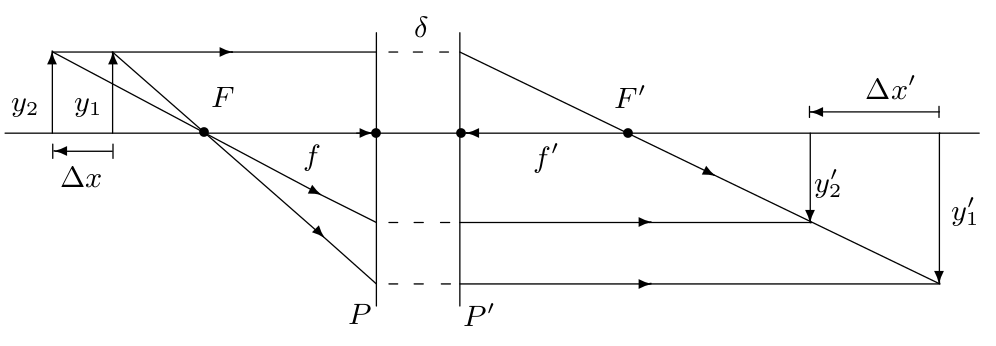
\includegraphics[width = 0.7\textwidth]{image/pic1.png}
    \caption{Измерение фокусного расстояния оптической
    системы по методу Аббе}
\end{figure}

\begin{table}[!ht]
    \centering
    \caption{Результаты измерения фокусного расстояния для линзы №1 по методу Аббе}
    \begin{tabular}{cccc}
    \hline
    \multicolumn{1}{|c|}{$x_1$, см}        & \multicolumn{1}{c|}{$x_1'$, см}      & \multicolumn{1}{c|}{$x_2$, см}        & \multicolumn{1}{c|}{$x_2'$,см}        \\ \hline
    \multicolumn{1}{|c|}{$27,50 \pm 0,05$} & \multicolumn{1}{c|}{$97,60\pm 0,05$} & \multicolumn{1}{c|}{$19,00 \pm 0,05$} & \multicolumn{1}{c|}{$67,80 \pm 0,05$} \\ \hline
    \multicolumn{1}{l}{}                   & \multicolumn{1}{l}{}                 & \multicolumn{1}{l}{}                  & \multicolumn{1}{l}{}                  \\ \hline
    \multicolumn{1}{|c|}{$y_1$, см}        & \multicolumn{1}{c|}{$y_1'$, см}      & \multicolumn{1}{c|}{$y_2$, см}        & \multicolumn{1}{c|}{$y_2'$,см}        \\ \hline
    \multicolumn{1}{|c|}{$2,00 \pm 0,05$}  & \multicolumn{1}{c|}{$7,80 \pm 0,05$} & \multicolumn{1}{c|}{$2,00 \pm 0,05$}  & \multicolumn{1}{c|}{$1,80 \pm 0,05$}  \\ \hline
    \end{tabular}
    \end{table}

    \noindent Рассчитаем фокусное расстояние $$f \approx 9,94 \pm 2,00 \;\text{см}.$$

    \subsection{Определение фокусного расстояния тонкой отрицательной линзы}

    Сначала с помощью собирающей линзы получим на экране действительное изображение предмета $S$ (точка $S_1$ на рис. 2). Затем на пути лучей, выходящих из собирающей линзы, расположим исследуемую рассеивающую линзу и, отодвигая экран, получим чёткое изображение предмета на экране, образованное двумя линзами.

    \begin{table}[!ht]
        \centering
        \caption{Результаты измерения фокусного расстояния для отрицательной линзы}
        \begin{tabular}{|c|c|c|}
        \hline
        $a_0$, см        & $a'$, см        & $l$, см          \\ \hline
        $42,10 \pm 0,05$ & $26,10\pm 0,05$ & $33,80 \pm 0,05$ \\ \hline
        \end{tabular}
        \end{table}

        Рассчитаем фокусное расстояние отрицательной линзы 
        $$\frac{1}{f_4} = -\frac{1}{a} + \frac{1}{a'},$$ 
        $$f_4 \approx  -12,17 \pm 1,05 \;\text{см}.$$


    \begin{figure}[ht!]
        \centering
        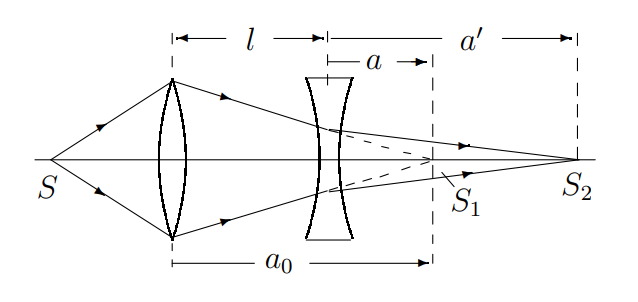
\includegraphics[width = 0.7\textwidth]{image/pic2.png}
        \caption{Измерение фокусного расстояния
        рассеивающей линзы}
    \end{figure}

    \subsection{Определение фокусных расстояний тонких линз с помощью зрительной трубы}

    Поставим собирающую линзу №1 на расстоянии от предмета, примерно равном фокусному расстоянию. На небольшом расстоянии от линзы закрепим трубу, настроенную на бесконечность, и отцентрируем её по высоте. Передвигая линзу вдоль скамьи и, если необходимо, перемещая линзу с помощью поперечных салазок, получим в окуляре зрительной трубы чёткое изображение предмета. При этом расстояние между предметом и серединой тонкой линзы (между проточками на оправах) равно фокусному расстоянию.

    \begin{table}[!ht]
        \centering
        \caption{Результаты измерений фокусных расстояний тонких линз с помощью зрительной трубы, где $f_1^1$ -- фокусное расстояние первой линзы до поворота, $f_1^2$ -- после поворота}
        \begin{tabular}{|c|c|c|}
        \hline
        $f_1^1$, см    & $f_1^2$, см    & $f_2$, см      \\ \hline
        $12,6 \pm 0,3$ & $12,7 \pm 0,3$ & $14,4 \pm 0,3$ \\ \hline
        \end{tabular}
        \end{table}

    \noindent По измеренным данным можно сказать, что собирающая линза № 1 является тонкой. \medskip

    \noindent Для определения фокусного расстояния тонкой рассеивающей линзы использем схему, изображённую на рис. 2. Сначала получим на экране увеличенное изображение предмета при помощи короткофокусной положительной линзы. Измерьте расстояние $a_0$ между линзой и экраном. Разместим сразу за экраном трубу, настроенную на бесконечность, и закрепим её. Уберём экран и поставим на его место исследуемую рассеивающую линзу. Отцентрируем световой пучок с помощью листа бумаги. Перемещая рассеивающую линзу, найдём в окуляре зрительной трубы резкое изображение предмета. Измерив расстояние $l$ между линзами, рассчитаем фокусное расстояние рассеивающей линзы в пространстве предметов $f = l - a_0$.

    \begin{table}[!ht]
        \centering
        \caption{Результаты определения фокусного расстояния тонкой рассеивающей линзы, где $f_4^1$ -- фокусное расстояние четвертой линзы до поворота, $f_4^2$ -- после поворота}
        \begin{tabular}{|c|c|c|c|c|}
        \hline
        $a_0$, см        & $l_1$, см        & $l_2$, см        & $f_4^1$, см     & $f_4^2$, см     \\ \hline
        $29,30 \pm 0,05$ & $14,80 \pm 0,05$ & $14,90 \pm 0,05$ & $-14,5 \pm 0,5$ & $-14,4 \pm 0,5$ \\ \hline
        \end{tabular}
        \end{table}

    \noindent Исходя из таблицы 4 можно сказать, что рассеивающая линза № 4 является тонкой.

    \newpage

    \subsection{Определение положения главных и фокальных плоскостей сложной оптической системы}

    Для нахождения главных плоскостей системы недостаточно знать
    фокусное расстояние, нужно определить ещё положения главных фоку-
    сов. Это можно сделать при помощи зрительной трубы, настроенной на
    бесконечность. Отложив от главных фокусов отрезки, равные фокусному расстоянию, можно найти положения главных плоскостей системы.При этом необходимо учитывать возможность различного взаимного расположения кардинальных точек (плоскостей) сложной системы. Результаты измерений представлены в таблице 5 и на рисунке~3.

    \begin{table}[!ht]
        \centering
        \caption{Результаты определения главных и фокальных плоскостей сложной оптической системы, где закрашенные ячейки были определены с помощью зрительной трубы}

        \begin{tabular}{|
        >{\columncolor[HTML]{DAE8FC}}c |
        >{\columncolor[HTML]{DAE8FC}}c |c|c|c|c|}
        \hline
        $F_{1\Sigma}$, мм & $F_{2\Sigma}$, мм & $f_{1\Sigma}$, мм & $f_{2\Sigma}$, мм & $F_{1\Sigma}$, мм & $F_{2\Sigma}$, мм \\ \hline
        $38,3 \pm 3$      & $35 \pm 3$        & $75 \pm 1$        & $75 \pm 1$        & $40 \pm 1$        & $33 \pm 1$        \\ \hline
        \end{tabular}
        \end{table}


\begin{figure}[!ht]
    \centering

\tikzset{every picture/.style={line width=0.75pt}} %set default line width to 0.75pt        

\begin{tikzpicture}[x=0.75pt,y=0.75pt,yscale=-1,xscale=1]
%uncomment if require: \path (0,300); %set diagram left start at 0, and has height of 300


%Straight Lines [id:da8929532668053957] 
\draw    (240,199.02) -- (240,64.02) ;
\draw [shift={(240,62.02)}, rotate = 90] [color={rgb, 255:red, 0; green, 0; blue, 0 }  ][line width=0.75]    (10.93,-3.29) .. controls (6.95,-1.4) and (3.31,-0.3) .. (0,0) .. controls (3.31,0.3) and (6.95,1.4) .. (10.93,3.29)   ;
\draw [shift={(240,201.02)}, rotate = 270] [color={rgb, 255:red, 0; green, 0; blue, 0 }  ][line width=0.75]    (10.93,-3.29) .. controls (6.95,-1.4) and (3.31,-0.3) .. (0,0) .. controls (3.31,0.3) and (6.95,1.4) .. (10.93,3.29)   ;
%Straight Lines [id:da33265633607059364] 
\draw    (383,200.02) -- (383,65.02) ;
\draw [shift={(383,63.02)}, rotate = 90] [color={rgb, 255:red, 0; green, 0; blue, 0 }  ][line width=0.75]    (10.93,-3.29) .. controls (6.95,-1.4) and (3.31,-0.3) .. (0,0) .. controls (3.31,0.3) and (6.95,1.4) .. (10.93,3.29)   ;
\draw [shift={(383,202.02)}, rotate = 270] [color={rgb, 255:red, 0; green, 0; blue, 0 }  ][line width=0.75]    (10.93,-3.29) .. controls (6.95,-1.4) and (3.31,-0.3) .. (0,0) .. controls (3.31,0.3) and (6.95,1.4) .. (10.93,3.29)   ;
%Straight Lines [id:da5007954898878026] 
\draw    (144,137) -- (144,127.02) ;
%Straight Lines [id:da23202446353175854] 
\draw  [dash pattern={on 4.5pt off 4.5pt}]  (39.28,133) -- (587.28,133) ;
%Straight Lines [id:da021251163389435668] 
\draw    (281,198.02) -- (281,63.02) ;
%Straight Lines [id:da11646988473253628] 
\draw    (323,196.02) -- (323,61.02) ;
%Straight Lines [id:da07828141030319791] 
\draw    (384,84) -- (529.28,84) ;
%Straight Lines [id:da5567553843453104] 
\draw  [dash pattern={on 0.84pt off 2.51pt}]  (277.28,84) -- (384,84) ;
%Straight Lines [id:da824520396317691] 
\draw    (41.28,161.02) -- (240.28,107.02) ;
%Straight Lines [id:da5319976294231632] 
\draw  [dash pattern={on 0.84pt off 2.51pt}]  (240.28,107.02) -- (356.28,77.02) ;
%Straight Lines [id:da9566214480393891] 
\draw    (478,137) -- (478,127.02) ;
%Straight Lines [id:da2944734776799147] 
\draw  [dash pattern={on 0.84pt off 2.51pt}]  (263.28,93.02) -- (383,115) ;
%Straight Lines [id:da37623146971221266] 
\draw    (383,115) -- (566.28,149.02) ;
%Straight Lines [id:da6353527620655999] 
\draw    (105,90) -- (238.28,90) ;

% Text Node
\draw (261,138) node [anchor=north west][inner sep=0.75pt]  [font=\scriptsize] [align=left] {$\displaystyle H_{1}$};
% Text Node
\draw (327,139) node [anchor=north west][inner sep=0.75pt]  [font=\scriptsize] [align=left] {$\displaystyle H_{2}$};
% Text Node
\draw (134,144) node [anchor=north west][inner sep=0.75pt]  [font=\footnotesize] [align=left] {$\displaystyle F_{1\Sigma }$};
% Text Node
\draw (466,144) node [anchor=north west][inner sep=0.75pt]  [font=\footnotesize] [align=left] {$\displaystyle F_{2\Sigma }$};


\end{tikzpicture}

\caption{Построение изображения в центрированной
оптической системе (приближенно)}

\end{figure}

\section{Вывод}

    В лабораторной работе были изучены различные методы определения фокусных расстояний линз. Также в ходе работы была определена <<тонкость>> линз (собирающей и рассеивающей --- см. таблицы 3 и 4). С помощью геометрического построения хода лучей были определены положения главных и фокальных плоскостей сложной оптической системы.

\end{document}
